\section{Refactoring} \label{sec:s4_refactoring}
%%% Intro paragraph --> Why do we refactor?

%%% How do we refactor?

%%% Summary --> Did the refactoring give us the desired results?

\subsection{Class Architecture}
In order to describe the structure design of the hotMap server, the UML v2.5 standard are used to express how the class hierarchy was designed. UML is a well known modeling language, for visualizing software system designs in order to more easily describe the static structure of a software system.
Therefore a UML class diagram are used for describing the model layer of the hotMap server.

Mixin is an language dependent functionality, which allows a class $A$ to contain methods from other classes or interfaces without having $A$ be a specialization of these other classes or traits. How class $A$ gain access to those methods through mixin are defined by the language. 

Scala does not have interfaces, but instead uses traits. These are similar but allow for default implementation of methods within the trait. When a concrete classes extends traits, it is called a realization of that trait, which in UML are indicated by a dashed arrow from the class to the interfaces. In scala traits can also be instantiated if all of its instance variables and methods have default implementions. In scala only traits can be mixed into classes or another trait.


In scala type aliases of mixin types are used to denoted a class or trait with a trait miexd into it. As an example of this we have on \cref{fig:class} that type $Point$ is a alias for any type which realizes the trait $Coordinate$ mixed with the trait $Weight$. UML cannot represent mixin, so it was chosen to show this by drawing a realization arrow with a mixin stereotype from the alias to the mixed type. Stereotypes are denoted by some text surrounded with $<<$ and $>>$ above the arrow.

\begin{sidewaysfigure}[htbp]
\centering
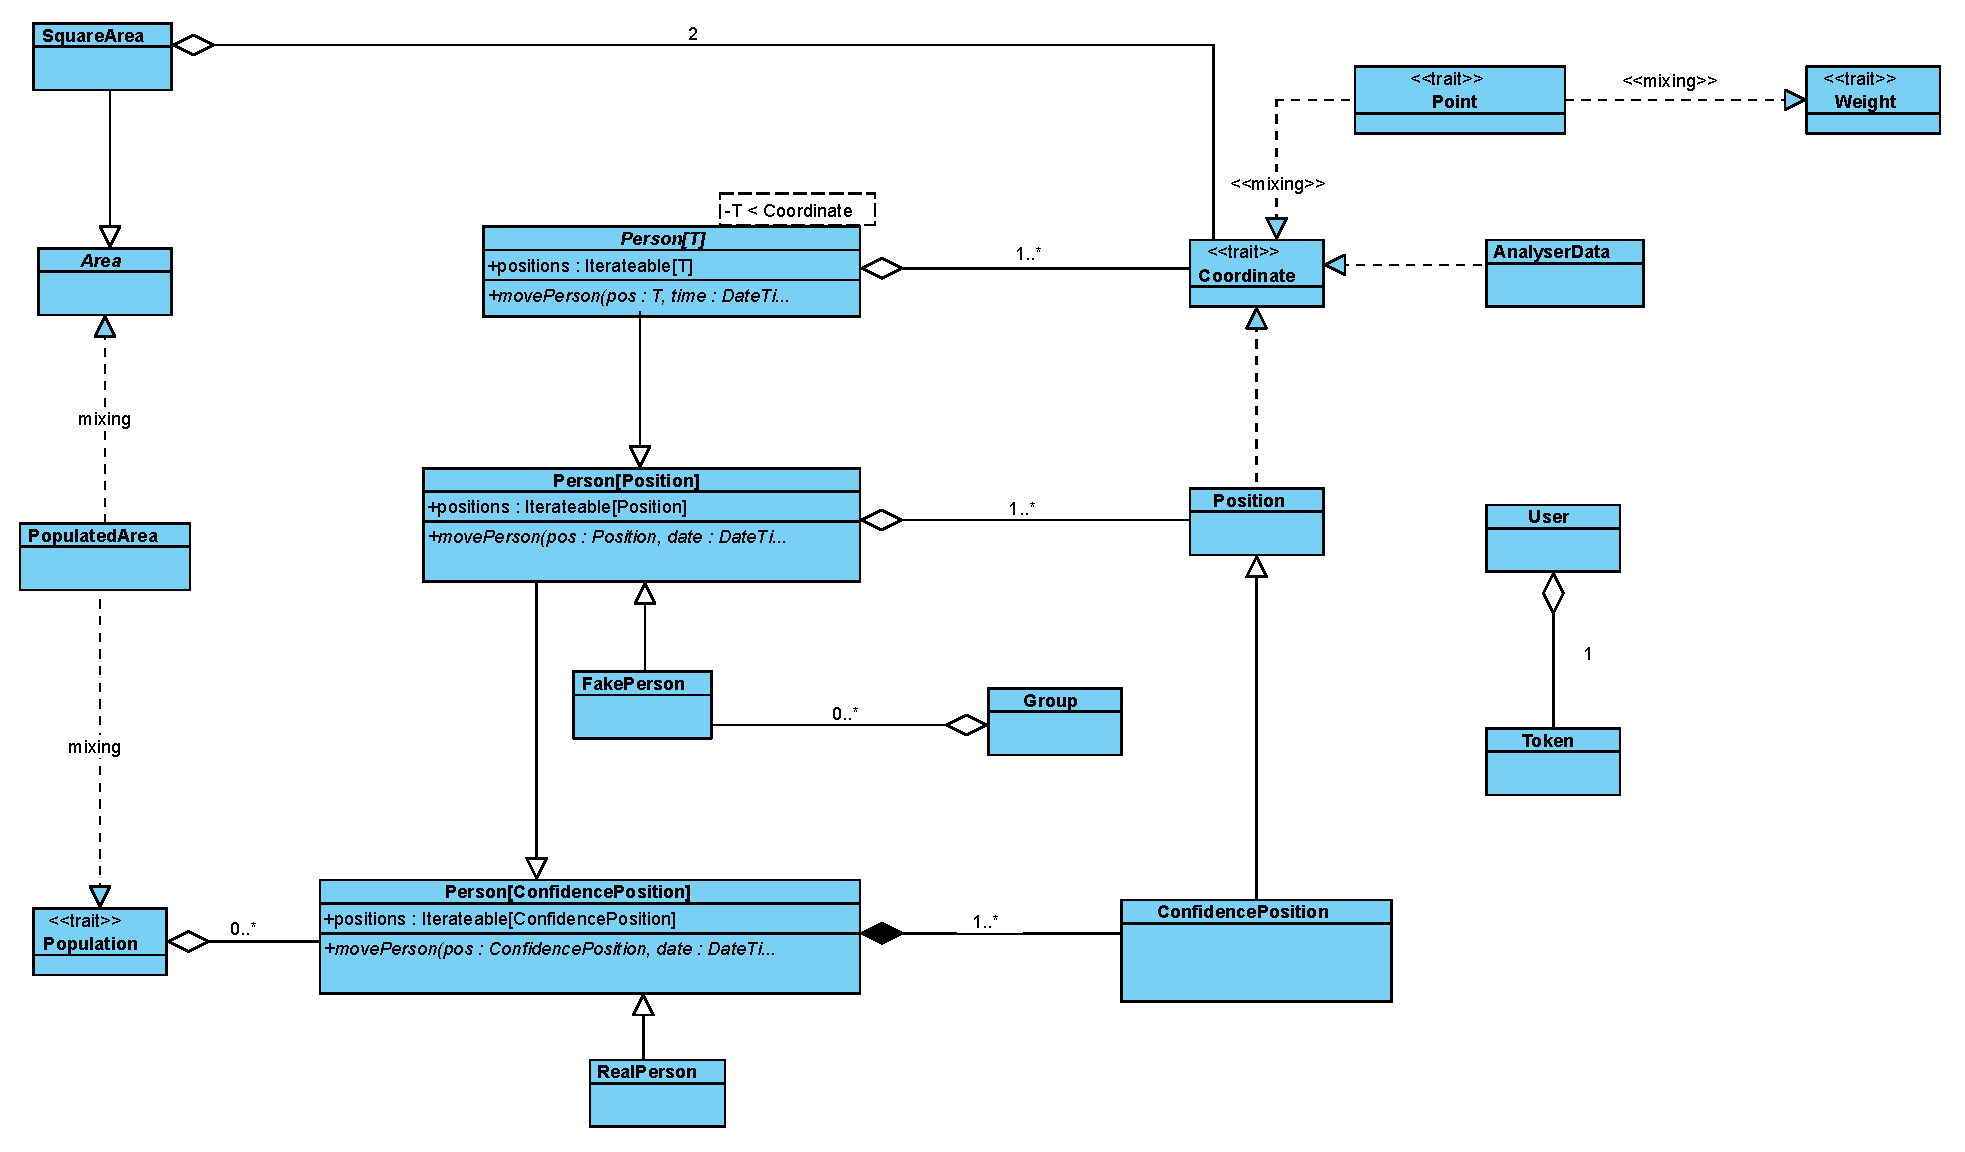
\includegraphics[width=\linewidth]{figures/class.eps}
\caption{Digraph.}
\label{fig:class}
\end{sidewaysfigure}


\subsection{Implementation of Asynchronous Analysis}
\label{sub:implementation_of_asynchronous_analysis}

As described in \cref{sub:Asynchronous_Analysis} the amount of calculations done can be reduced by analysing asynchronously from user requests, and store completed analyses. We assume that mostly users will monitor real-time crowd factors, therefor we will focus on optimizing real-time analyzing.

This was implemented using a infinite loop running on another thread, which fetches and analyses position data from the astep core. Completed Analysis's from this thread are stored in a global variable. When a user requests crowd factors the request handler will respond with data obtained from this global variable. There are one thread which writes data to the global variable, and potentially one thread per user reading data from this global variable. The global variable is a pointer to the result of the latest completed Analysis, and when new data is completely analyzed this pointer is changed atomically to prevent race conditions. 

The infinite loop are repeated at most once per 5 seconds, in case an iteration of the loop takes longer than 5 seconds the next iteration will not start until the previous has completed. The 5 seconds limitation are set because the astep core cannot deliver data any faster. One iteration on the loop consists of 5 stages which are described in the following enumeration. 

\begin{enumerate}
    \item \textbf{Fetch position data} This stage fetches position data from the astep core.
    \item \textbf{Process the position data} At this stage all the fetched positions are associated with the corresponding person based on a id revised together with every position. This id identifies a single single WiFi device. Afterwards the method $moverPerson$ are called for every instance of the class Person with the corresponding new position as parameter in order to add this position to a persons history.
    \item \textbf{Calculate analyses data} The purpose of this stage is to calculates a List of $AnalyserData$ for each $Area$. This involves calculating all persons heading direction and velocity and encapsulate this in to an instance of the class $AnalyserData$.
    \item \textbf{Analysis} This stages analyses the data from the last stage for estimating  crowd factors of each $Area$.
    \item \textbf{JSON Conversion} At the last stage the result of the analysis are converted in to JSON, which then are stored in the global variable for use upon user requests. 
\end{enumerate}

In summary this technique ensures that the process of analyzing data will not run for every users request of real-time information, which improves performance on the server. It also improves client side performance because request of analyzed data takes less time. Another advantage of this technique is that multiple users monitoring real-time crowd conditions will be shown the exact same information.
